
\documentclass{article}
\usepackage[spanish]{babel} %Definir idioma español
\usepackage[utf8]{inputenc} %Codificacion utf-8
\usepackage{amssymb, amsmath, amsbsy, wasysym}
\usepackage{multirow} % para tablas
\usepackage{graphicx}
\usepackage{listings}
\usepackage{hyperref}
\title{Tarea 3\\Control inteligente}
\author{Emmanuel Peto Gutiérrez}
\begin{document}
\maketitle

En esta práctica se realizó control sobre un tanque de agua con una bomba de entrada y un orificio de salida. En este se usó control con un sistema de inferencia borroso de Takagi-Sugeno (\textit{fuzzy inference system}).

\section{Sistema de inferencia borroso (FIS)}

El primer paso es hacer borroso el error, el cual será el valor de entrada del FIS. Para esta práctica se considerará que el error está en el rango [-2 2] y se calcula como $h_0 - h$, donde $h_0$ es la altura objetivo y $h$ la altura actual del agua.

Para los valores en los extremos se usaron las funciones de pertenencia $z$ y $s$, en los intervalos de [-2 -0.75] y [0.75 2], respectivamente. Para los valores intermedios (entre -1 y 1) se usaron 5 funciones de pertenencia gaussianas. En la siguiente figura se observan las funciones de pertenencia respecto al valor del error.

\begin{center}
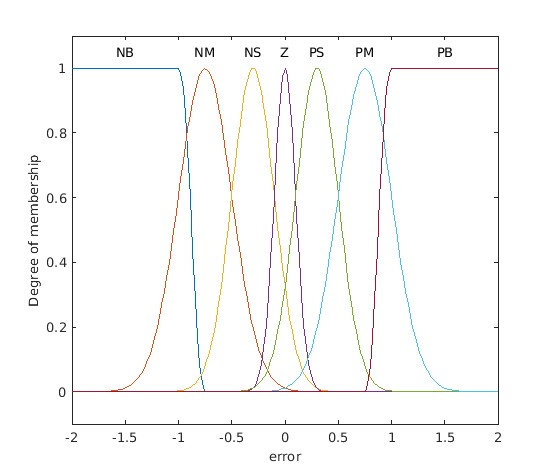
\includegraphics[scale=0.4]{membership}
\end{center}

La salida del sistema serán dos valores: $V_1$ y $V_2$. En un sistema de Takagi-Sugeno la salida puede ser una función lineal de la entrada, o bien, una constante. En este caso las salidas son solo constantes y se utiliza la siguiente nomenclatura:

\begin{itemize}
\item FDR $\rightarrow$ 0 (fuera de rango).
\item Z $\rightarrow$ 0.25, (cerca del cero).
\item S $\rightarrow$ 0.5 (pequeño).
\item M $\rightarrow$ 0.75 (mediano).
\item B $\rightarrow$ 1 (grande).
\end{itemize}

Las reglas del sistema son las siguientes.

\begin{tabular}{|c|c|c|}
\hline
\textbf{error} & \textbf{$V_1$} & \textbf{$V_2$} \\ \hline
NB & FDR & B \\ \hline
NM & FDR & M \\ \hline
NS & FDR & S \\ \hline
Z & Z & Z \\ \hline
PS & S & FDR \\ \hline
PM & M & FDR \\ \hline
PB & B & FDR \\ \hline
\end{tabular}

Finalmente, podemos ver una gráfica del sistema de Takagi-Sugeno generado.

\begin{center}
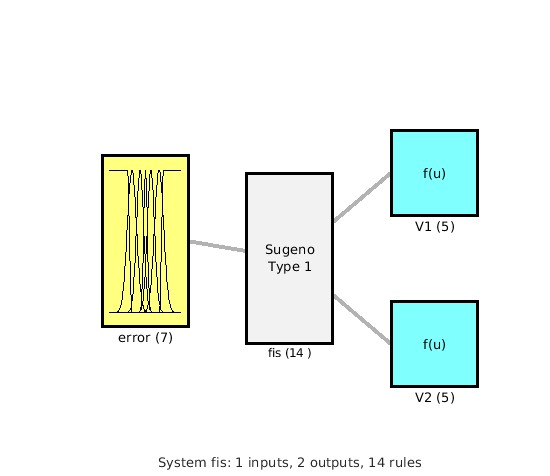
\includegraphics[scale=0.5]{sugeno}
\end{center}

El script de Matlab del sistema de control borroso es \texttt{sugeno\_tank.m}, lo cual genera un archivo de salida \texttt{error\_tanque.fis}.

\section{Modelo del tanque}

La altura del tanque respecto al tiempo se describe con la siguiente ecuación diferencial $$ \frac{dh}{dt} = V_1 q_e - V_2 \sqrt{h} $$ donde $q_e$ es el flujo de entrada (fijado en 1), $h$ es la altura actual, $V_1$ es la fracción de apertura de la válvula de entrada y $V_2$ la fracción de apertura de la válvula de salida.

El modelo del tanque para Simulink se obtuvo de \url{https://la.mathworks.com/help/slcontrol/gs/watertank-simulink-model.html} y se describe mediante la siguiente figura

\begin{center}
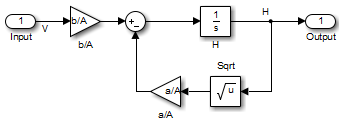
\includegraphics[scale=1]{op_watertank_subsystem}
\end{center}

Excepto que se cambia $b/A$ por $V_1$ y $a/A$ por $V_2$ para que la notación sea igual a la de nuestro problema.

\section{Control borroso}

El sistema de control borroso se modela con el siguiente diagrama de Simulink

\begin{center}
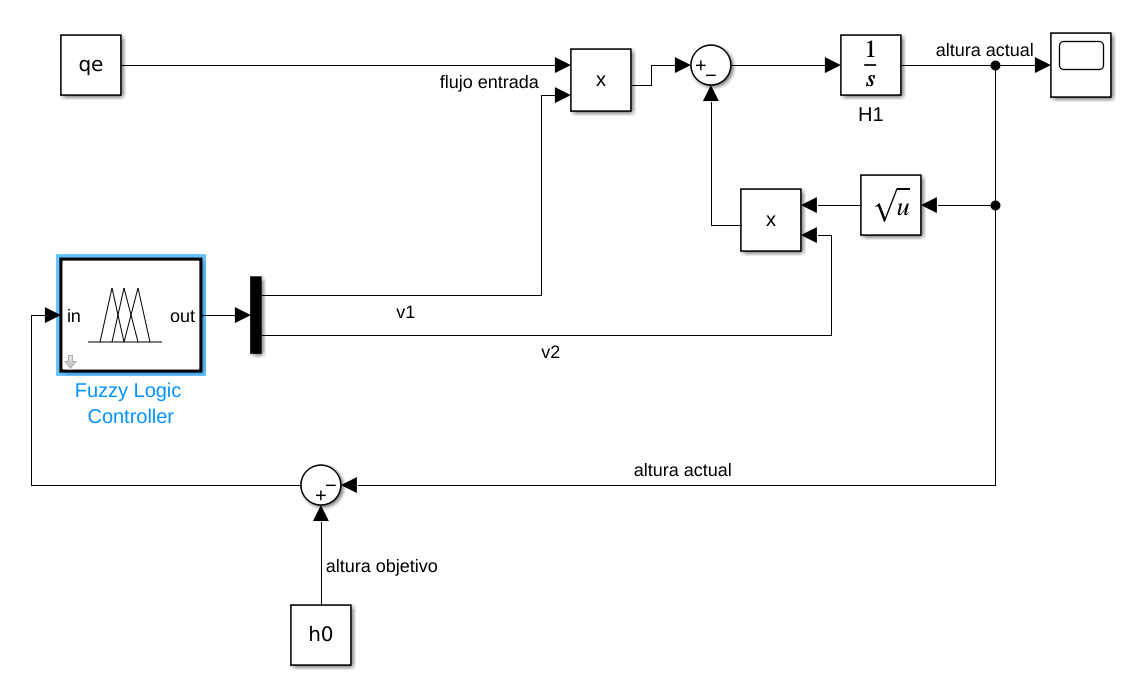
\includegraphics[width=\linewidth]{diagrama_fuzzy_control}
\end{center}

La altura objetivo se fijó en $h_0$ = 2m. Primero se realizó el experimento cuando el nivel del tanque está por debajo del objetivo (1 m), y la gráfica del control borroso se observa en la siguiente figura. El eje $x$ es el tiempo en segundos y el eje $y$ es la altura del tanque.

\begin{center}
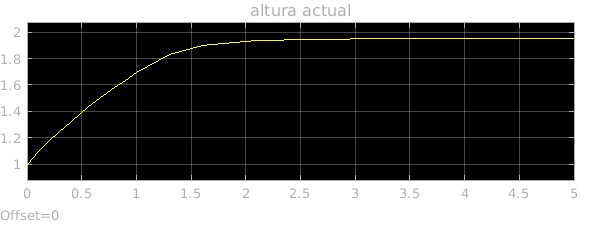
\includegraphics[width=\linewidth]{altura1}
\end{center}

Se observa que la altura del tanque se acerca al 2 (el objetivo) en aproximadamente 2.5 segundos y de ahí se mantiene en equilibro, sin alcanzar ni rebasar el 2.

Luego, se realizó el experimento con una altura mayor al objetivo (4 m). La gráfica de la altura del tanque respecto al tiempo es la siguiente.

\begin{center}
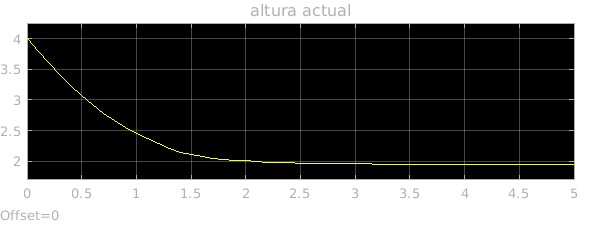
\includegraphics[width=\linewidth]{altura4}
\end{center}

Se observa que el nivel del tanque baja de 4 a 2 en aproximadamente 2 segundos; luego baja un poco del 2 y de ahí se mantiene en equilibrio.

\end{document}

